\section{Linear Discriminant Analysis}

Linear discriminant analysis(LDA) is a supervised classification method used to separate classes of data by linear decision boundaries. Each decision boundary is a hyperplane $H$ from which the minimum distance from the classes it separates is maximized, and the distance from the means of the classes are maximized. A decision boundary is defined as a linear combination of the feature values x and is given as:

\begin{equation}
g(x) = w^tx +w_0
\end{equation}

where $w$ is a weight vector deciding the orientation of $H$, and $w_0$ is a bias deciding the position of the hyperplane in relation to the origin. In a two category case the decision rule for deciding class $w_1$ or $w_2$ is: decide $w_1$ if $g(x) > 0$ and $w_2$ if $g(x) < 0$. $g(x) = 0$ then defines the decision boundary that separates the features into two decision regions $R_1$ for $w_1$ $R_2$ for $w_2$. $w$ is normal (orthogonal) to any vector on $H$, which can be used to calculate the distance $r$ from feature values to the decision boundary:

\begin{equation}
r = \frac{g(x)}{||w||}
\end{equation} 

From origin the distance is given as $\frac{w_0}{||w||}$, where if $w_0 > 0$ the origin is on the positive side of the decision surface, and if $w_0 < 0$ the origin is on the negative side. In the case of $w_0 = 0$ the decision surface passes through origin. In \figref{geolda} a geometric illustration of the linear discriminant function and its properties  is depicted.

\begin{figure}[H]                 
	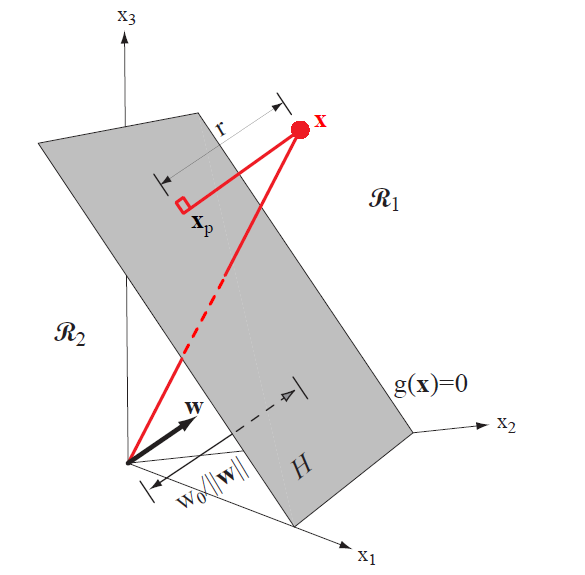
\includegraphics[width=.4\textwidth]{figures/xBackground/geolda}  
	\caption{A geometric illustration of the linear decision surface $g(x)$ that separates the feature space into two decision regions $R_1$ and $R_2$. \cite{Duda2000}}
	\label{fig:geolda} 
\end{figure}

In a multicategory case $c$ decision boundaries are defined. The approach for defining the decision boundaries is given as:

\begin{equation}
	g_{i}(x) = w^tx_i +w_{i0} ~~~~~~~~~~~ i = 1,...,c,
\end{equation}

where $x$ is assigned to $w_i$ if $g_i(x) > g_i(x)$ for all $j \neq i$. This type of classifier is called a linear machine, and will be adopted as classification method in this project. 


\subsection{Generalized discriminant function}


\subsection{Gradient descend/minimum criterion function}


\subsection{Classification scores}
Evaluating the certainty that a feature value belongs to a given class can be done by computing the posterior probability of each class. The posterior probability is a value between 0 and 1, and is calculated as follows:

\begin{equation}
P(w_j|x) = \frac{P(x|w_j)P(w)}{P(x)}
\end{equation}

, where $w_j$ represents a class and x represents a feature value. The posterior probability is given as the product of the class conditional probability, $P(x|w_j)$ and the prior $P(w)$ divided by a normalization term $P(x)$ that guaranties that the posterior probabilities for all classes sums to one. $P(x|w_j)$ is the probability of obtaining a feature value when selecting samples randomly from a class. $P(w)$ is the likelihood that a sample from a class appears compared to the other class before it actually has appeared. 
